\documentclass[a4paper,12pt]{article}

% Packages for language and font settings
\usepackage[utf8]{inputenc}  % For UTF-8 encoding
\usepackage[T1]{fontenc}     % For better font encoding
\usepackage[english]{babel}  % For English language

% Packages for formatting
\usepackage{geometry}        % To customize page layout
\geometry{a4paper, margin=1in}

\usepackage{setspace}        % For line spacing
\onehalfspacing              % Set 1.5 line spacing

\usepackage{parskip}         % Adds space between paragraphs

% Packages for headers and footers
\usepackage{fancyhdr}
\pagestyle{fancy}
\fancyhf{}
\fancyhead[L]{\textbf{Lab Report}} % Left header
\fancyhead[R]{\thepage}            % Right header


% Packages for math and symbols
\usepackage{amsmath, amssymb, amsfonts} % Advanced math
\usepackage{siunitx}                    % For SI units

% Packages for tables and figures
\usepackage{graphicx}                   % For images
\usepackage{caption}                    % For customizing captions
\usepackage{subcaption}                 % For subfigures
\usepackage{booktabs}                   % For professional-quality tables
\usepackage{array}                      % For custom table columns
\usepackage{float}
% Packages for referencing
\usepackage{hyperref}                   % Hyperlinks
\hypersetup{
    colorlinks=true,
    linkcolor=blue,
    citecolor=blue,
    urlcolor=blue,
    pdftitle={Lab Report },
    pdfauthor={Your Name},
}

\usepackage{biblatex}                   % For bibliography management
\addbibresource{references.bib}         % Specify your bibliography file

% Packages for code
\usepackage{listings}                   % Code highlighting
\usepackage{xcolor}                     % Custom colors for listings

\lstset{
    frame=single,
    numbers=left,
    numberstyle=\tiny\color{gray},
    basicstyle=\ttfamily\small,
    keywordstyle=\color{blue},
    stringstyle=\color{red},
    commentstyle=\color{gray},
    breaklines=true,
}

% Custom Commands
\newcommand{\vect}[1]{\mathbf{#1}}      % Shortcut for vectors
\newcommand{\dif}{\mathrm{d}}           % Differential symbol
% Title Page
\title{\textbf{Lab Report 2}}
\author{Sai Akhila Reddy Turpu - EE24BTECH11055 \\Suguru Sai Akshita - EE24BTECH11054 }

\date{\today}

% Begin Document
\begin{document}

\maketitle
\tableofcontents
\newpage

\section{Objective}

1. Analyzing the RC circuit response for square wave input\\
\section{Apparatus and procedure}
\subsection{Materials}
\begin{itemize}
    \item Cathode ray Oscilloscope
    \item Function Generator (2 channels)
    \item Probes
    \item Connecting wires
    \item Breadboard
    \item Capacitor $1 \mu $F
    \item Resistor $(1\text{k}\Omega)$
\end{itemize}


\begin{figure}[h]
    \centering
    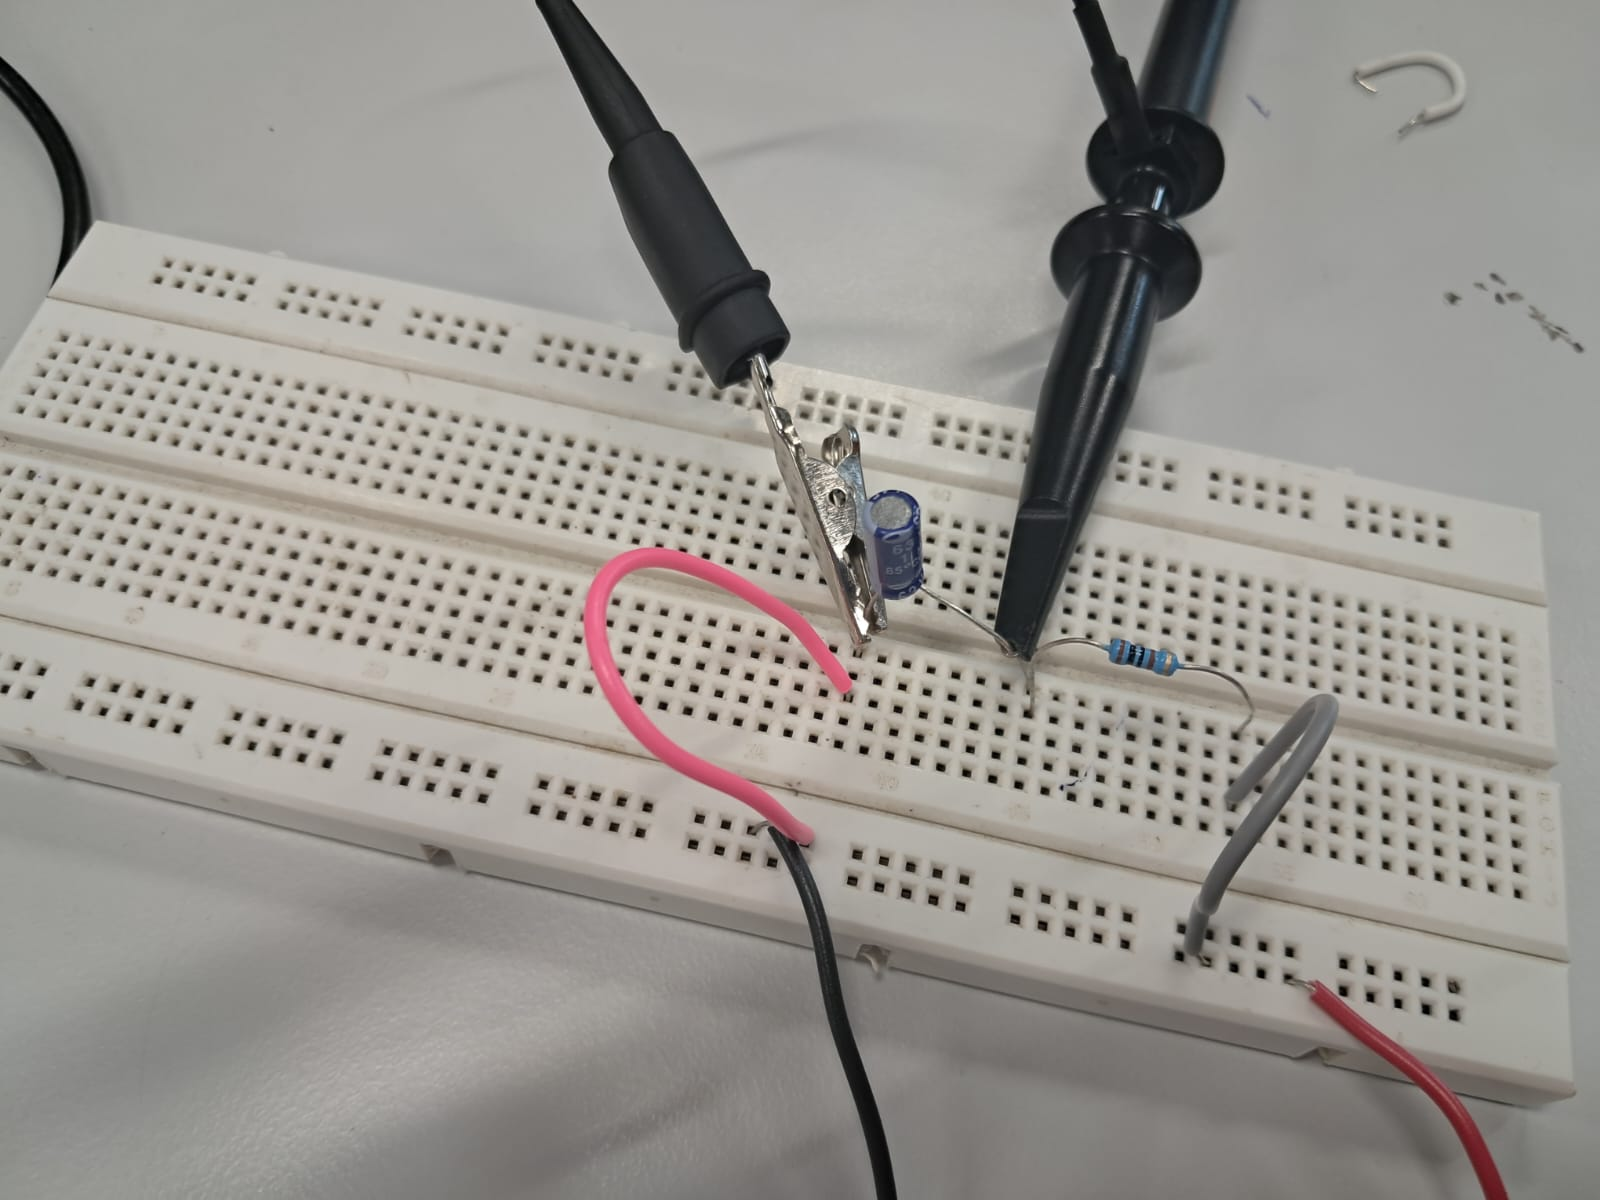
\includegraphics[width=\textwidth]{figs/circuit.jpeg}
\end{figure}




\subsection{Procedure}

\begin{enumerate}
    \item Place the Components on the Breadboard:

Insert the electrolytic capacitor into the breadboard. Ensure the longer leg (positive) and shorter leg (negative) are correctly oriented.

Insert the resistor into the breadboard, ensuring one end connects to the capacitor.
     \item Connect Power Supply:

Use red and black wires to provide power to the circuit.

The red wire is connected to the positive rail.

The black wire is connected to the negative rail (ground).
    \item Connect one end of the resistor to the capacitor.

Connect the other end of the resistor to the designated node (gray wire area).
   \item Attach the black probe to the ground of the circuit.

Attach the second probe to the capacitor-resistor junction to monitor the signal.
   \item Observe the circuit operation and monitor signals using the oscilloscope. Adjust the frequency accordingly for observations.

   \item Press Mode/Coupling button and then change sweep mode from auto to normal.
   In the Trigger menu, press Mode until “Edge” is selected.
   Then select Single mode. Wait until mode will initiate.

   \item Set the number of cycles to $5$ and push the trigger to generate the transient response. 

    \item Now, change the mode to continuous and wait for $1$ second to obtain the steady state response.

    \item Keep changing the frequency to get different responses. 
    
\end{enumerate}

\section{Observation}
$RC=10^{-3}$\\
We have 3 cases:
\begin{enumerate}
    \item $T>>RC$
     \item $T=RC$
      \item $T<<RC$
\end{enumerate}

\subsection{T$>>$RC  ($T=10$ ms)}
For the input shown in the figure below, the output signal recorded on the oscilloscope is as follows:
\begin{figure}[h]
    \centering
    \begin{minipage}{0.45\textwidth}
        \centering
        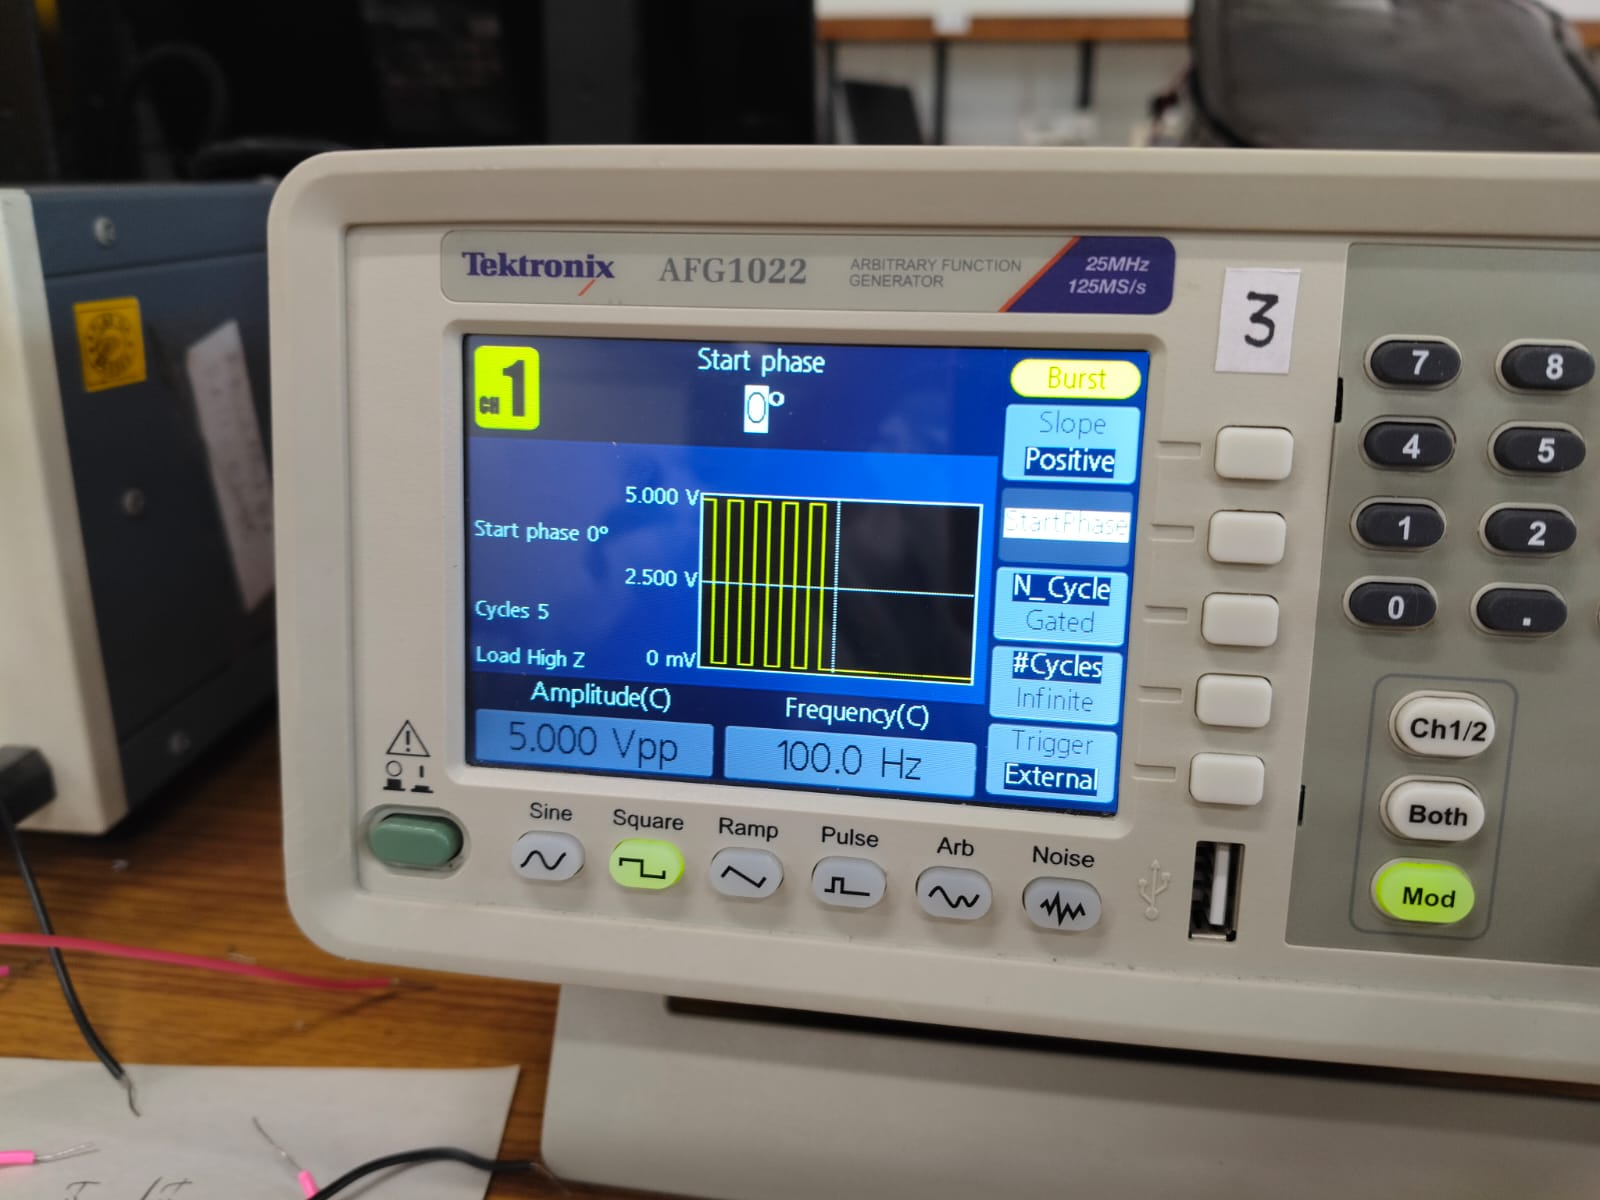
\includegraphics[width=\textwidth]{figs/T100para.jpeg}
    \end{minipage}\hfill
    \begin{minipage}{0.45\textwidth}
        \centering
        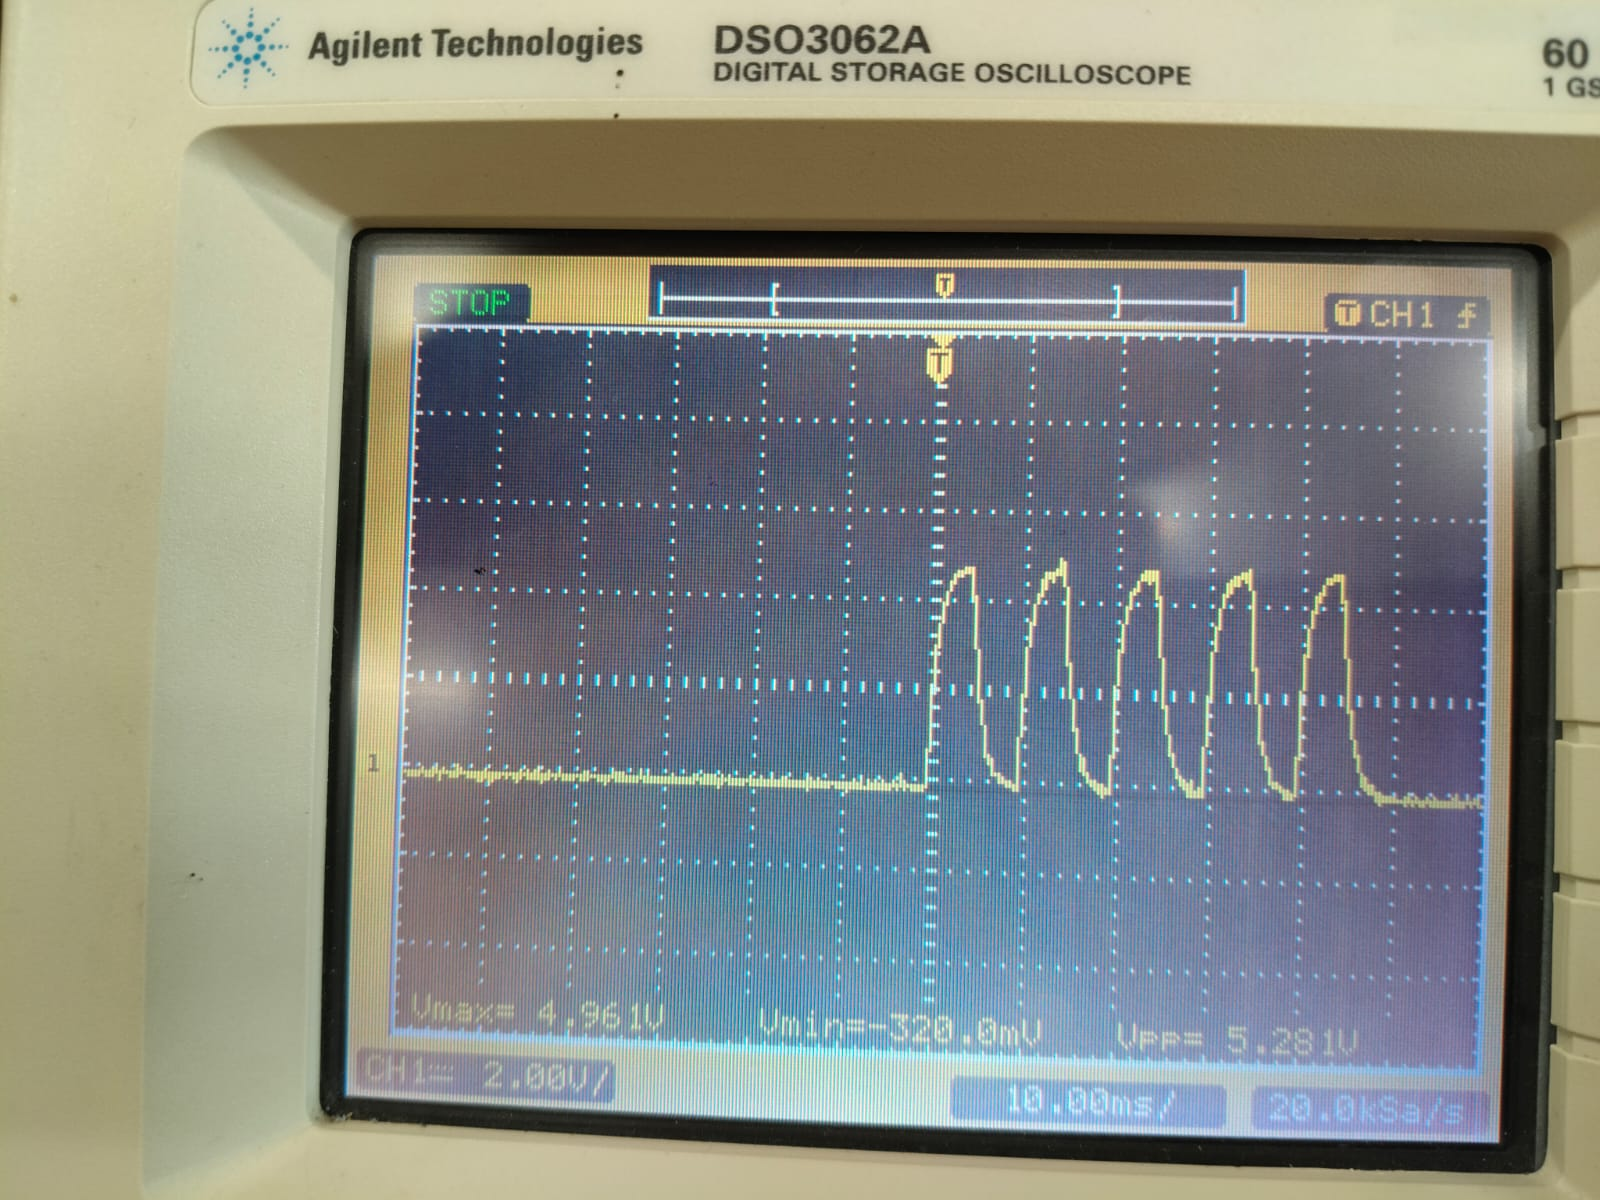
\includegraphics[width=\textwidth]{figs/T100plot.jpeg}
    \end{minipage}
\end{figure}


\textbf{Explanation:}
The equation for charging of a capacitor is given by:
$$V_1=V_0(1-e^{-\frac{t}{\tau}})$$
$$V_1=5(1-e^{-\frac{10^{-2}}{2\times 10^{-3}}})$$
$$V_1=5(1-e^{-5})$$
$$V_1=4.966$$
Now the maximum value of the first peak is $4.96$V. 
Now, as the value of the signal from the function generator is zero, the capacitor starts discharging, with the peak value as $1.96$V.
The equation for discharging of a capacitor is:
$$V=V_0e^{-\frac{(t-(T/2))}{\tau}}$$
$$V_2=4.966 \times e^{-\frac{t-10^{-2}/2}{10^{-}}}$$
$$V_2=4.966 \times e^{-\frac{10^{-2}-10^{-2}/2}{10^{-3}}}$$
$$V_2=0.0334606$$
Now, we again send a signal of $5$V.
On solving the differential equation corresponding to a series RC circuit with initial conditions, we get:\\
$$v=V(1-e^{-\frac{t-t_0}{RC}})+v_0e^{-\frac{(t-t_0)}{RC}}$$
Here, $v_0=0.0334606$\\
Hence, 
$V_3=5(1-e^{-5})+0.0335(e^{-5})$
$$V_3=4.966225$$
We notice that $V_3 > V_1$.
Again, now when the capacitor starts discharging, we get,
$$V_4=V_3e^{-\frac{t-(3T/2)}{\tau}}$$
$$V_4=0.03346216$$
In the same way, we calculate the values of $V_5$, $V_6$ and so on.\\
As the number of cycles increases, the circuit is most likely going to reach steady state.
Given below is the steady state response of the circuit:
\begin{figure}[h]
    \centering
    \begin{minipage}{0.45\textwidth}
        \centering
        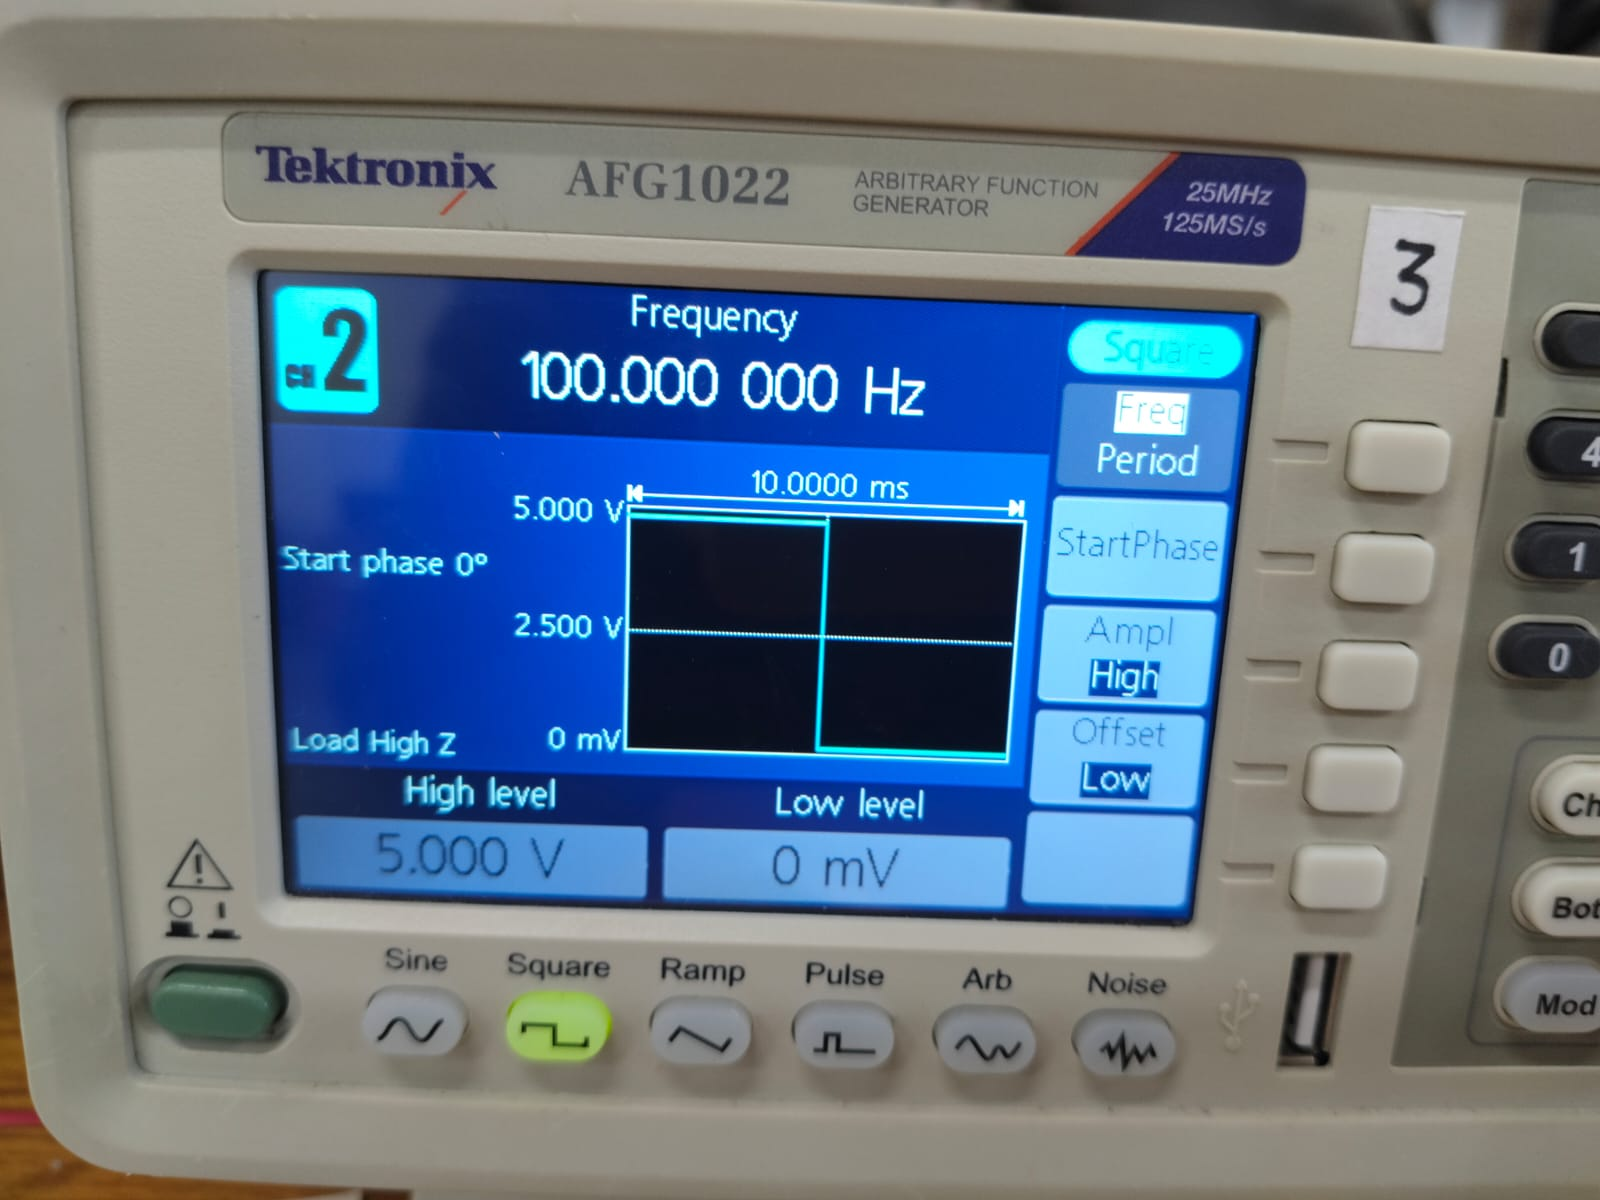
\includegraphics[width=\textwidth]{figs/C100para.jpeg}
    \end{minipage}\hfill
    \begin{minipage}{0.45\textwidth}
        \centering
        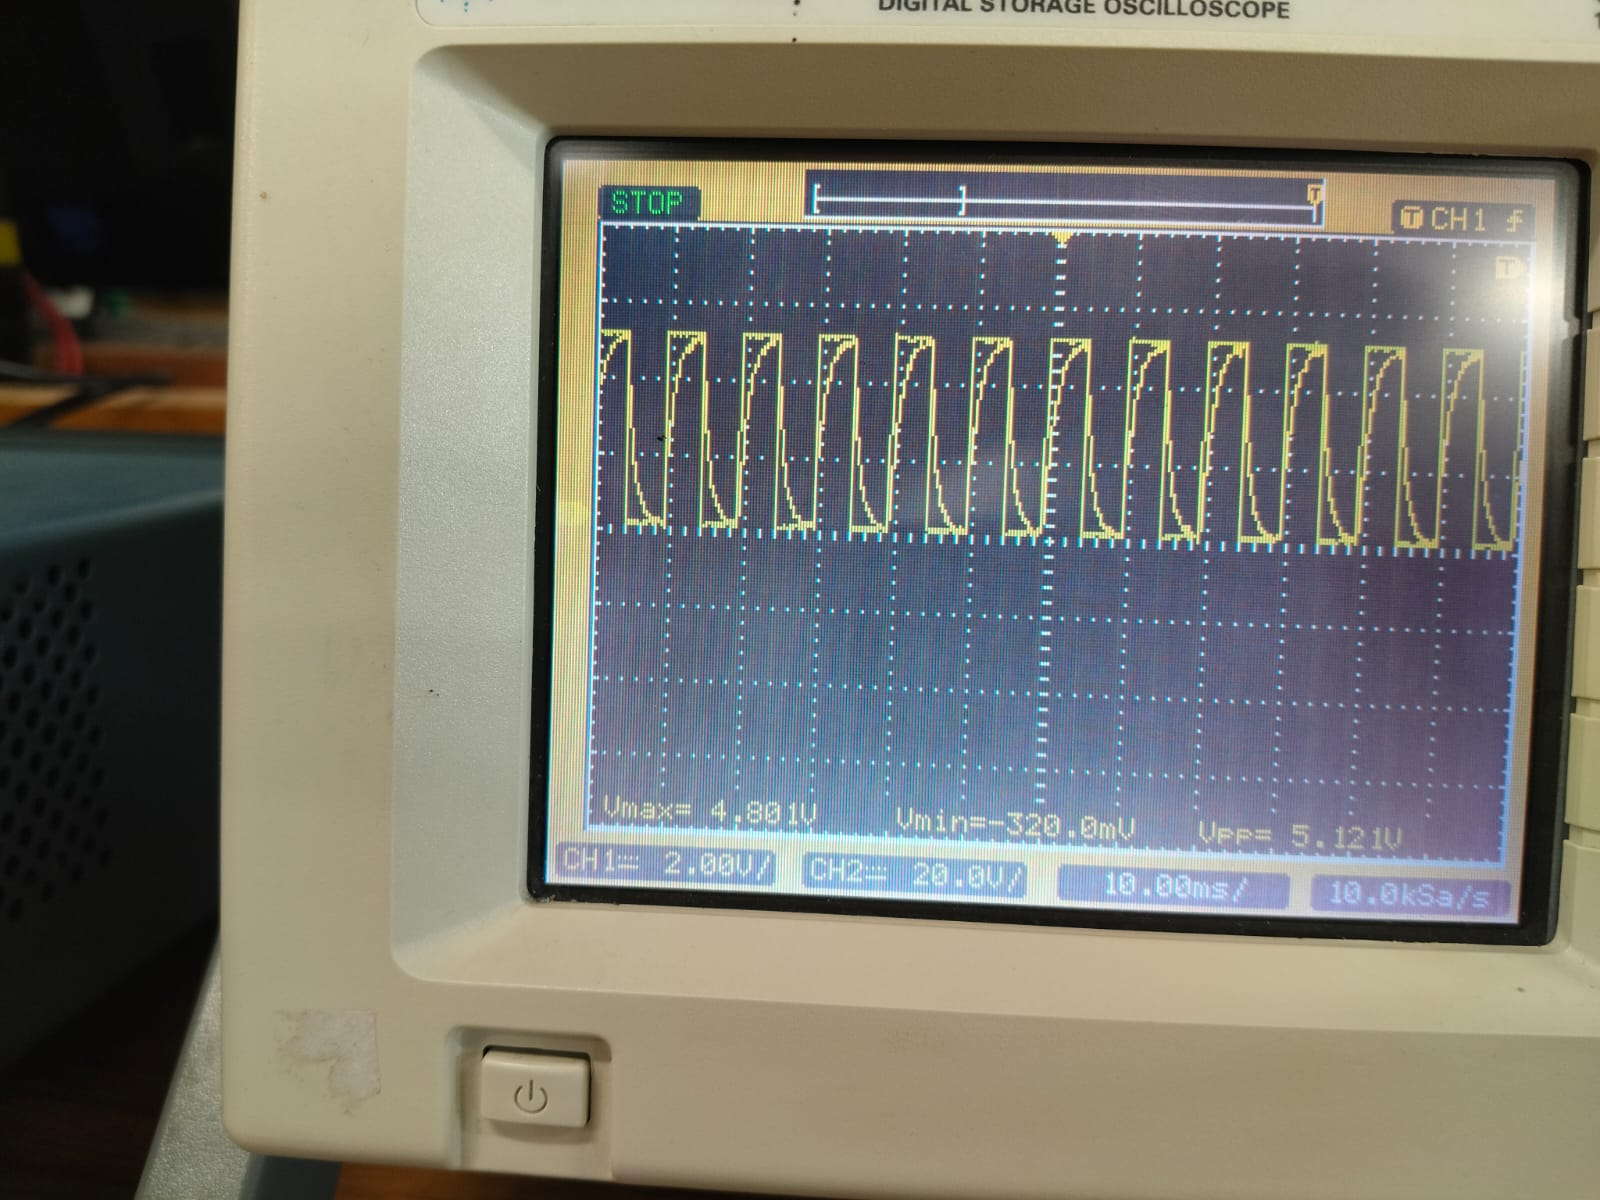
\includegraphics[width=\textwidth]{figs/C100plot.jpeg}
    \end{minipage}
\end{figure}



\subsection{T$=$RC ($T=1$ms)}
For the input shown in the figure below, the output signal recorded on the oscilloscope is as follows:

\begin{figure}[h]
    \centering
    \begin{minipage}{0.45\textwidth}
        \centering
        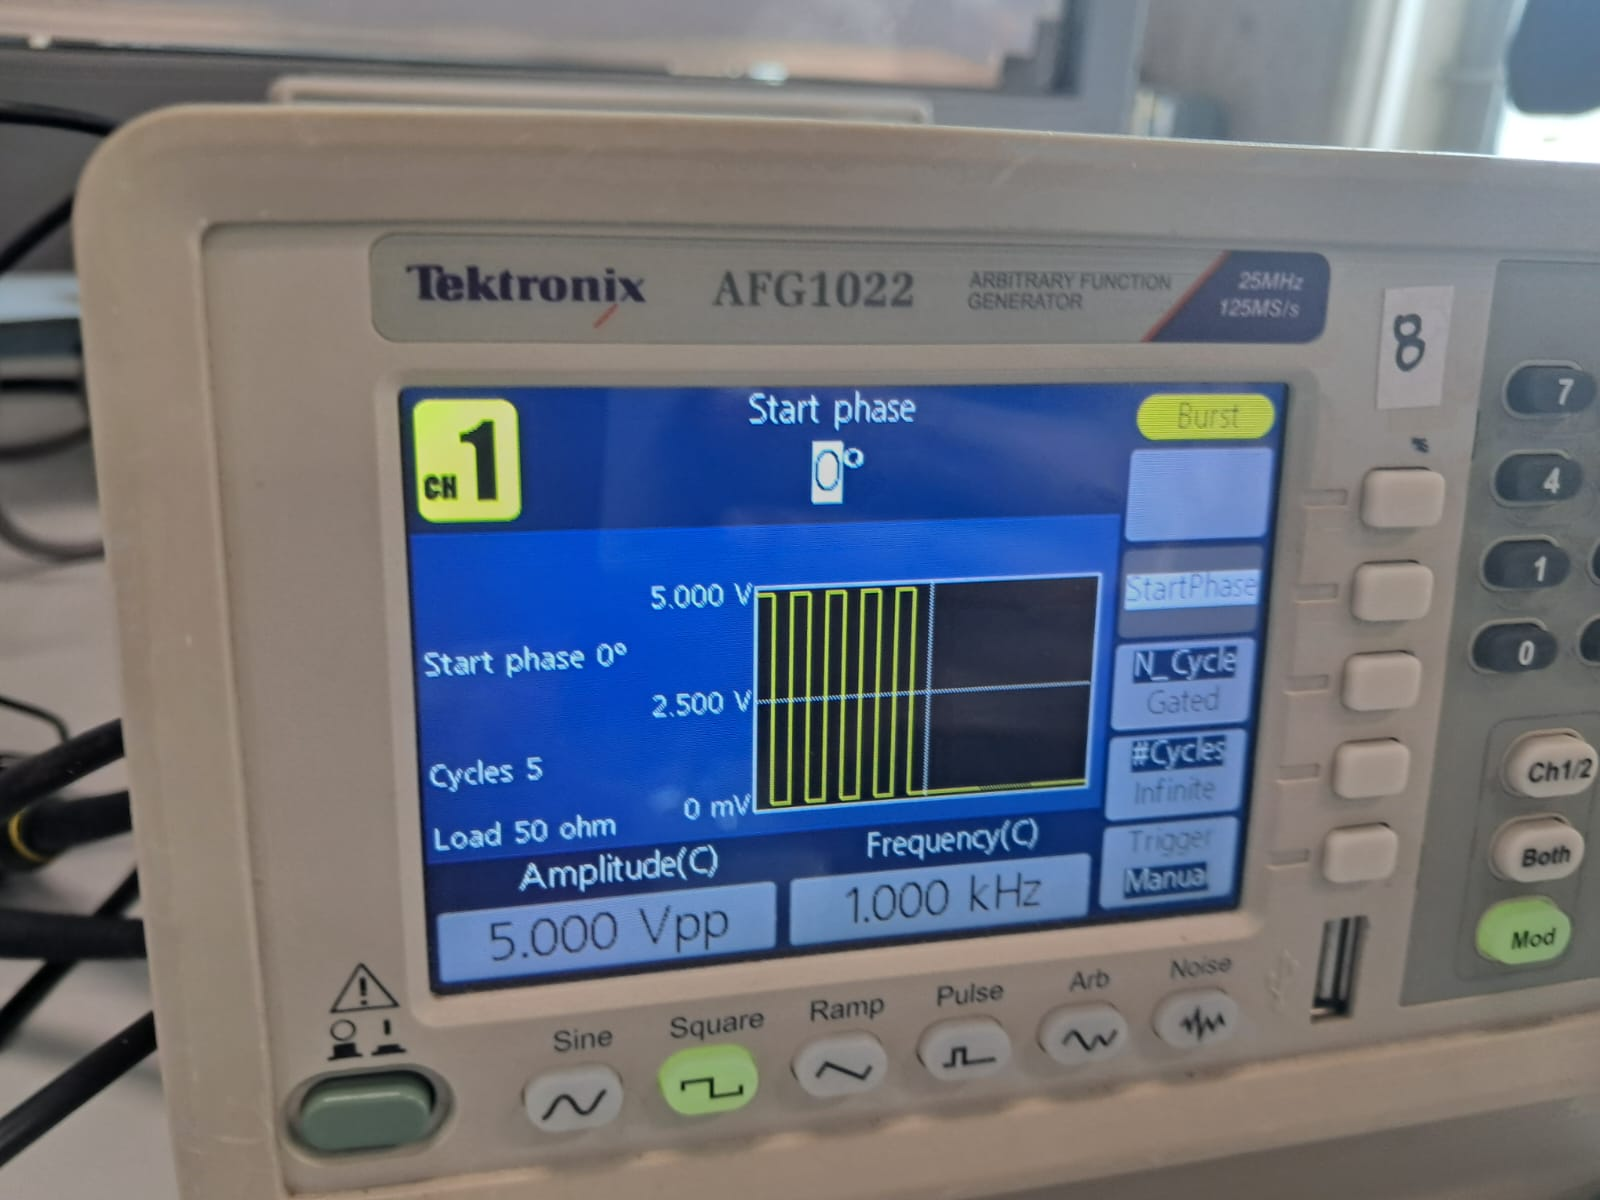
\includegraphics[width=\textwidth]{figs/T1kpara.jpeg}
    \end{minipage}\hfill
    \begin{minipage}{0.45\textwidth}
        \centering
        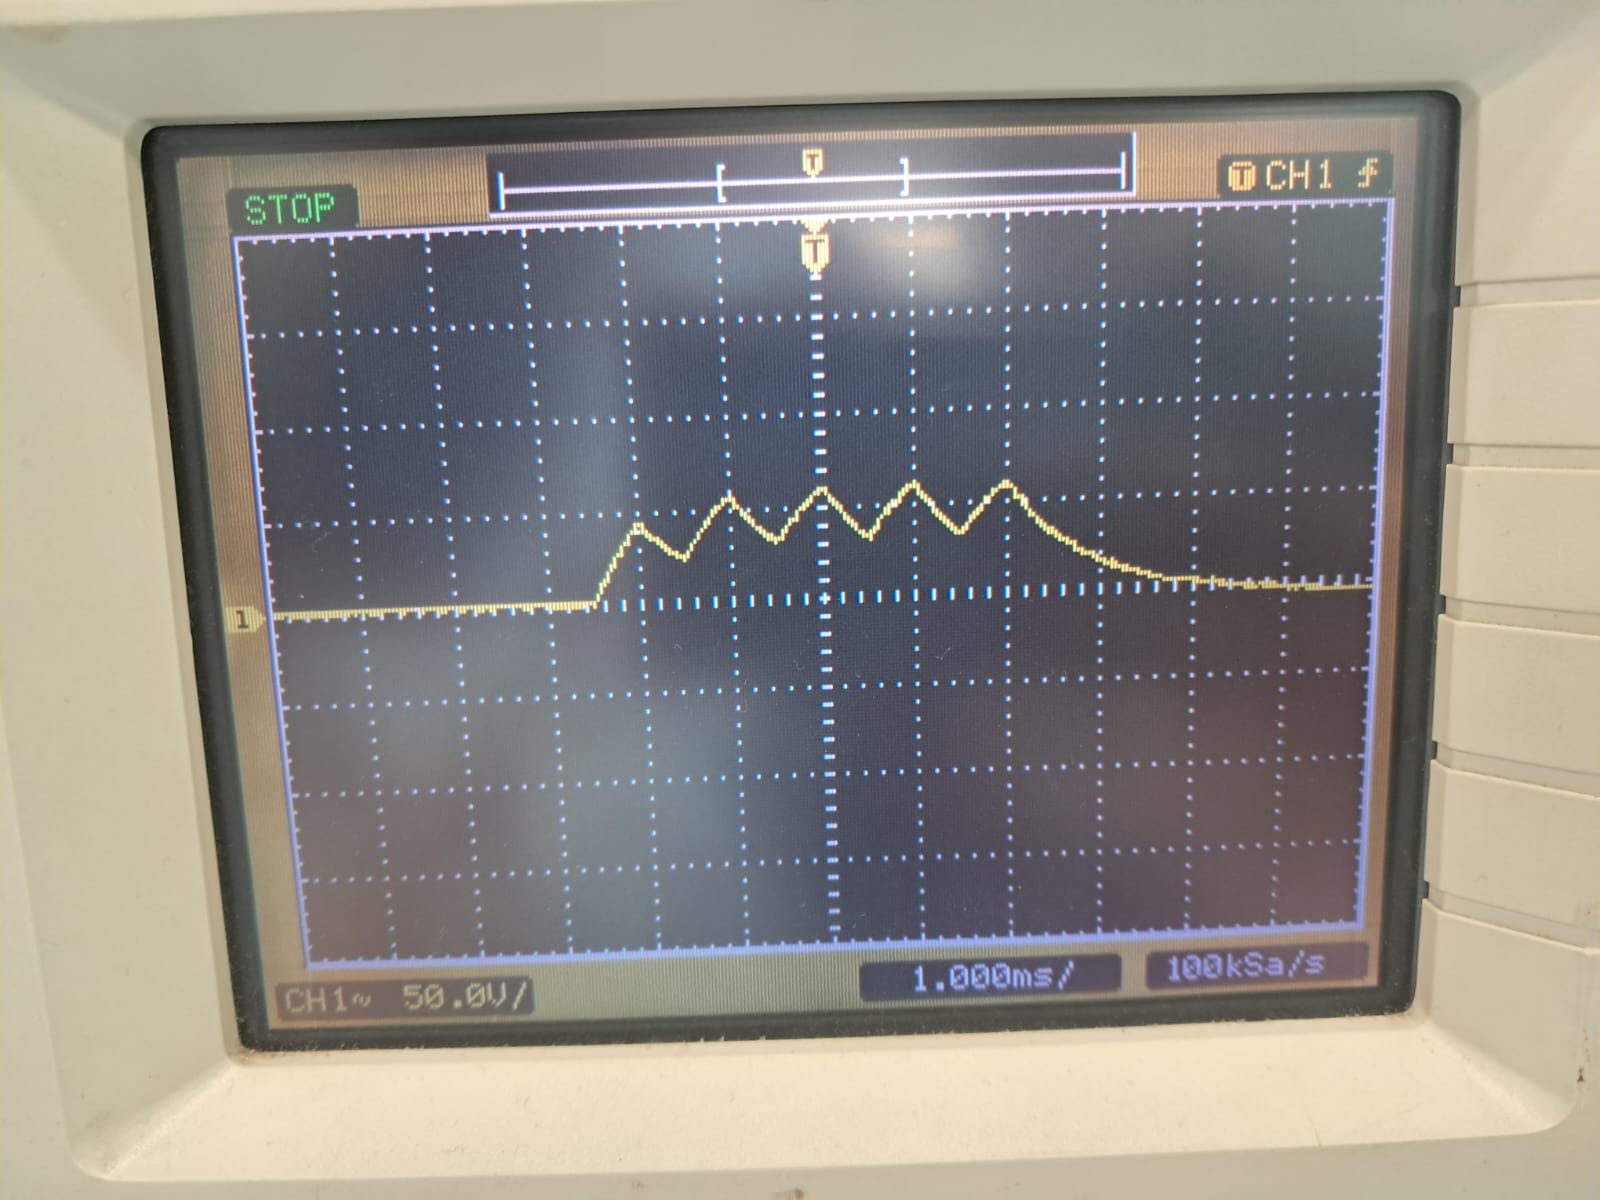
\includegraphics[width=\textwidth]{figs/T1kplot.jpeg}
    \end{minipage}
\end{figure}


\textbf{Explanation:}
The equation for charging of a capacitor is given by:
$$V_1=V_0(1-e^{-\frac{t}{\tau}})$$
$$V_1=5(1-e^{-\frac{10^{-3}}{2\times 10^{-3}}})$$
$$V_1=5(1-e^{-\frac{1}{2}})$$
$$V_1=1.96$$
Now the maximum value of the first peak is $1.96$V. 
Now, as the value of the signal from the function generator is zero, the capacitor starts discharging, with the peak value as $1.96$V.
The equation for discharging of a capacitor is:
$$V=V_0e^{-\frac{(t-(T/2))}{\tau}}$$
$$V_2=1.96 \times e^{-\frac{t-10^{-3}/2}{10^{-3}}}$$
$$V_2=1.96 \times e^{-\frac{10^{-3}-10^{-3}/2}{10^{-3}}}$$
$$V_2=1.193$$
Now, we again send a signal of $5$V.
On solving the differential equation corresponding to a series RC circuit with initial conditions, we get:\\
$$v=V(1-e^{-\frac{t-t_0}{RC}})+v_0e^{-\frac{(t-t_0)}{RC}}$$
Here, $v_0=1.193$\\
Hence, 
$V_3=5(1-\frac{1}{\sqrt{e}})+1.193(\frac{1}{\sqrt{e}})$
$$V_3=2.691$$
We notice that $V_3 > V_1$.
Again, now when the capacitor starts discharging, we get,
$$V_4=V_3e^{-\frac{t-(3T/2)}{\tau}}$$
$$V_4=1.632$$
In the same way, we calculate the values of $V_5$, $V_6$ and so on.\\
As the number of cycles increases, the circuit is most likely going to reach steady state.
\begin{align}
    V_5&=2.957\\
    V_6&=1.794\\
    V_7&=3.055\\
    V_8&=1.8532\\
    V_9&=3.091\\
    V_{10}&=1.875\\
    V_{11}&=3.1042
\end{align}
Given below is the steady state response of the circuit:

\begin{figure}[h]
    \centering
    \begin{minipage}{0.45\textwidth}
        \centering
        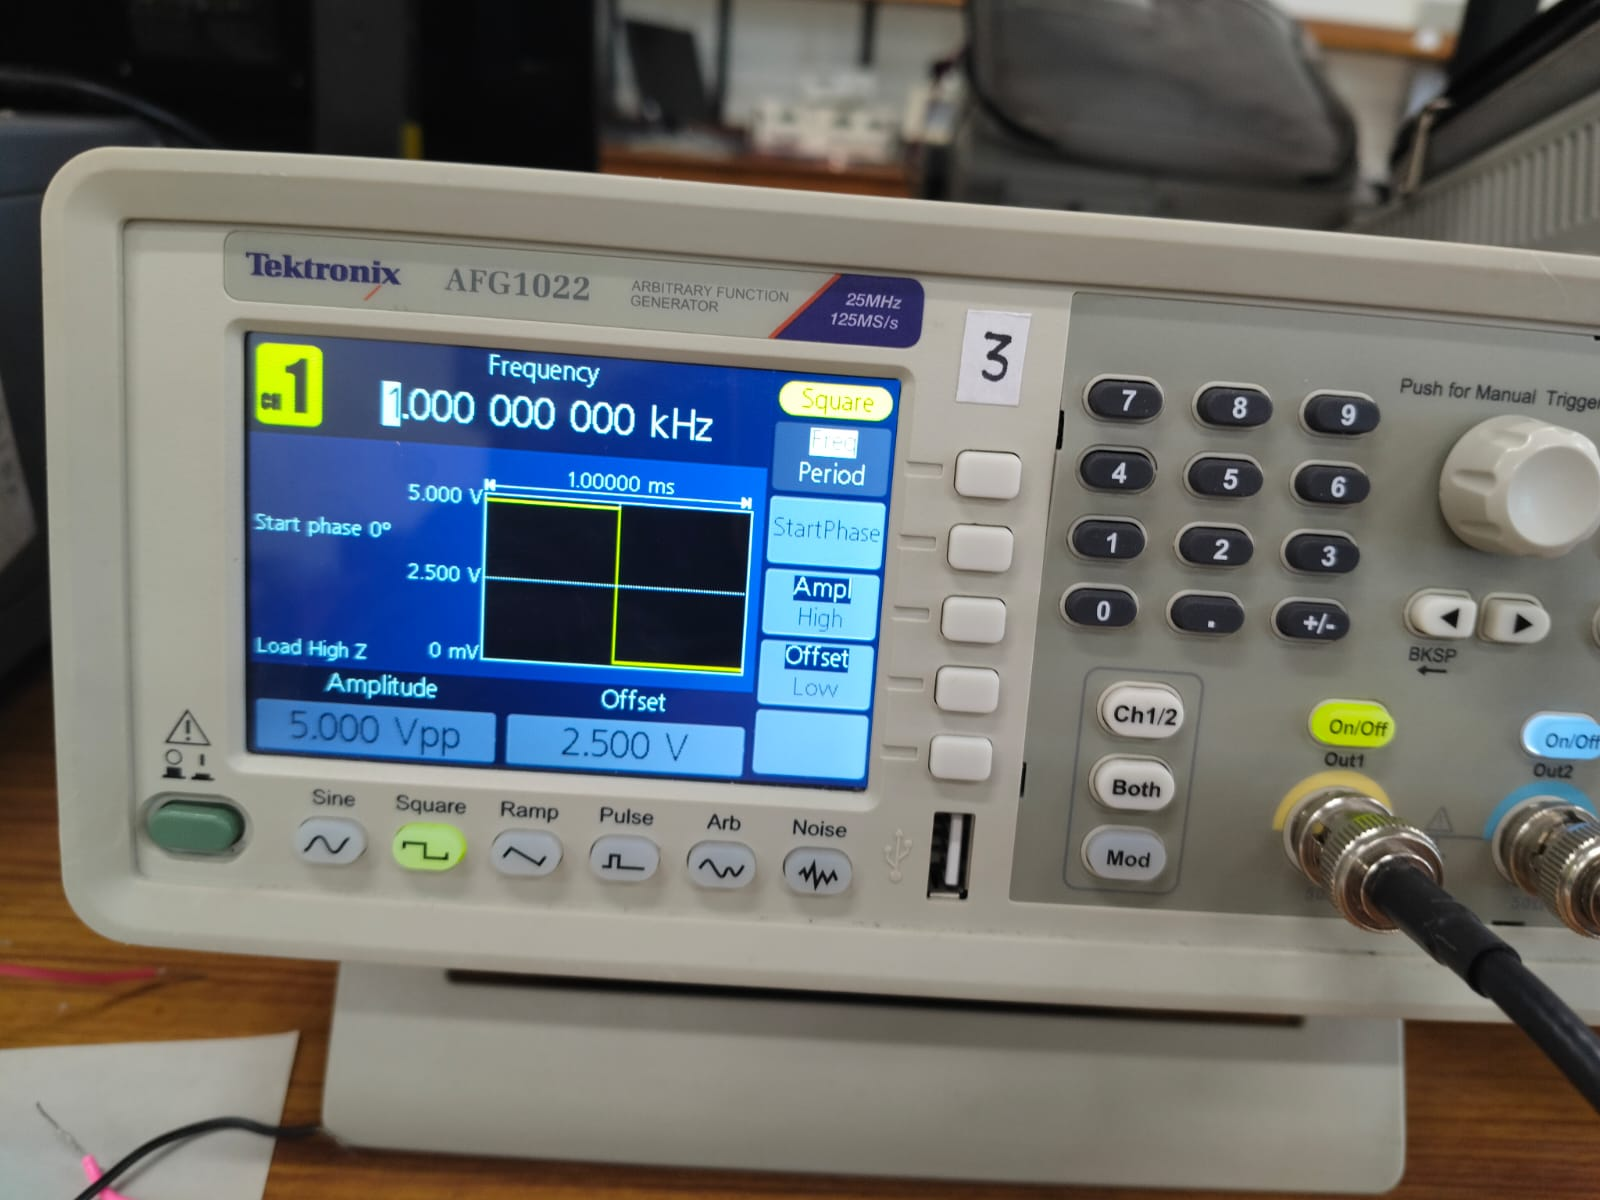
\includegraphics[width=\textwidth]{figs/C1kpara.jpeg}
    \end{minipage}\hfill
    \begin{minipage}{0.45\textwidth}
        \centering
        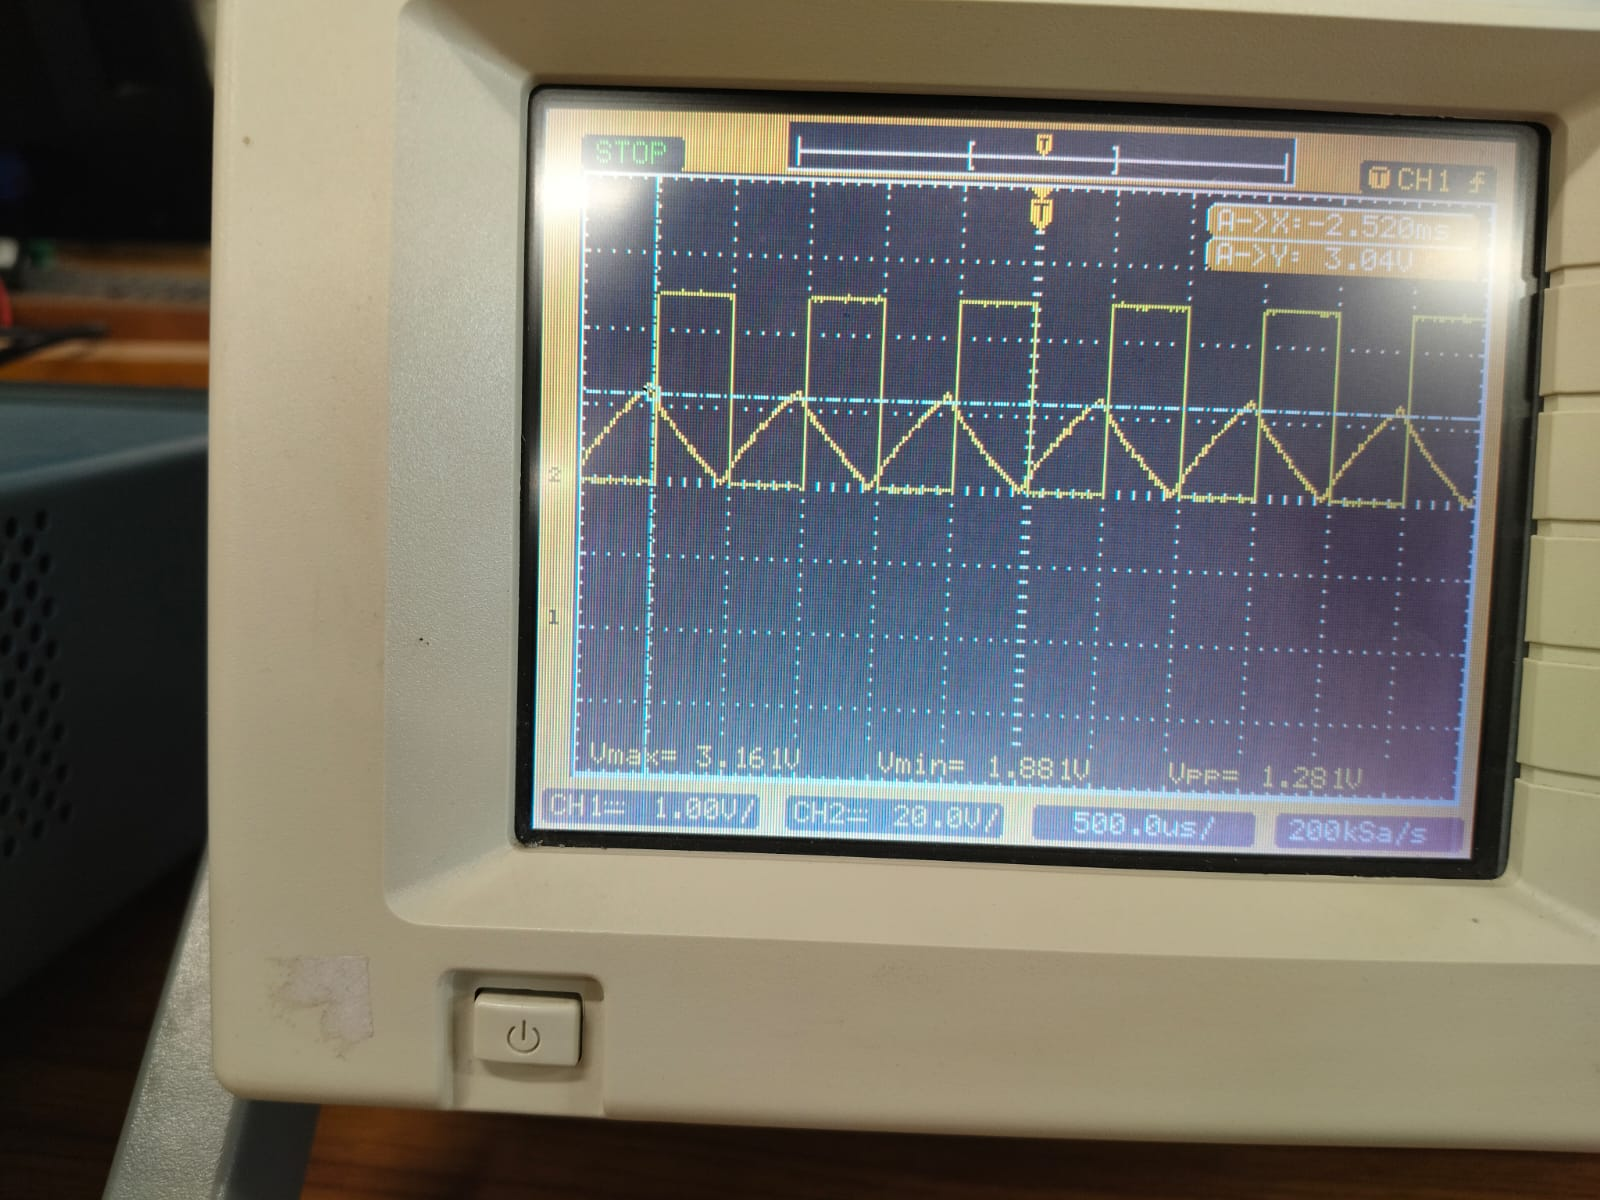
\includegraphics[width=\textwidth]{figs/C1kplot.jpeg}
    \end{minipage}
\end{figure}



\subsection{T$<<$RC ($T=0.5$ ms)}
For the input shown in the figure below, the output signal recorded on the oscilloscope is as follows:

\begin{figure}[h]
    \centering
    \begin{minipage}{0.45\textwidth}
        \centering
        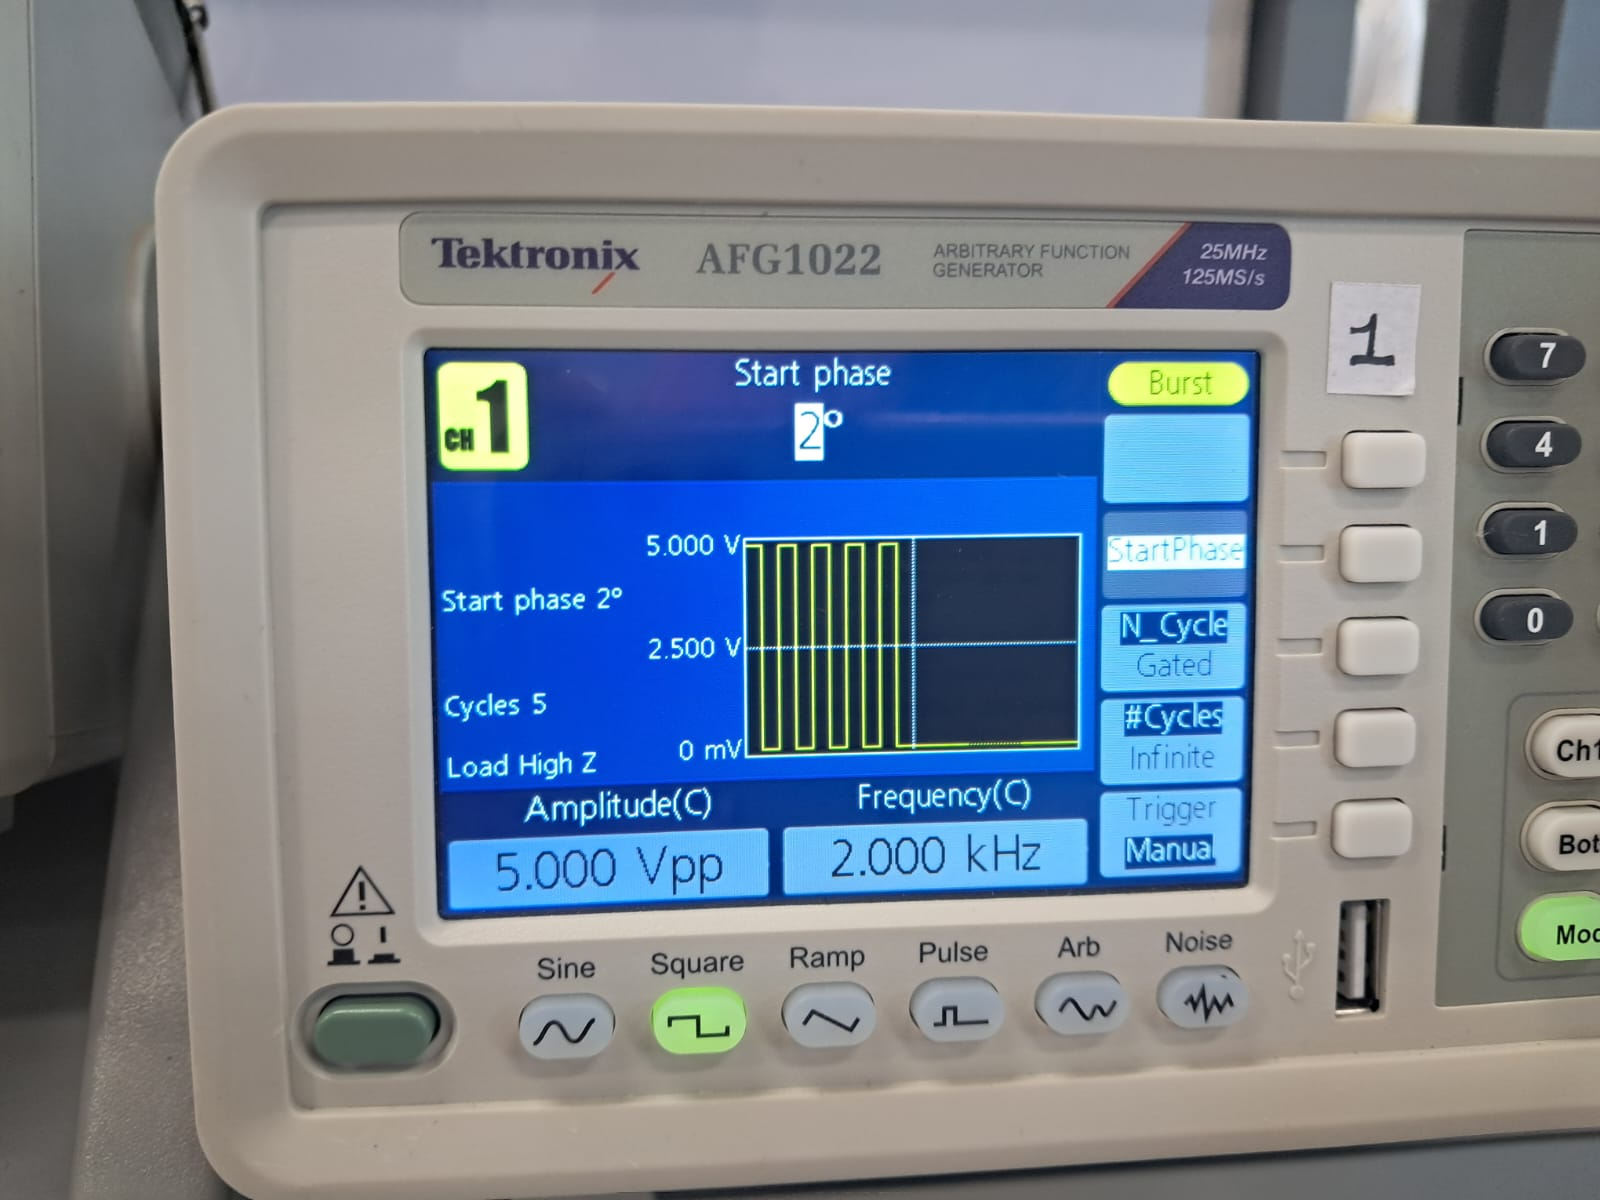
\includegraphics[width=\textwidth]{figs/T2kpara.jpeg}
    \end{minipage}\hfill
    \begin{minipage}{0.45\textwidth}
        \centering
        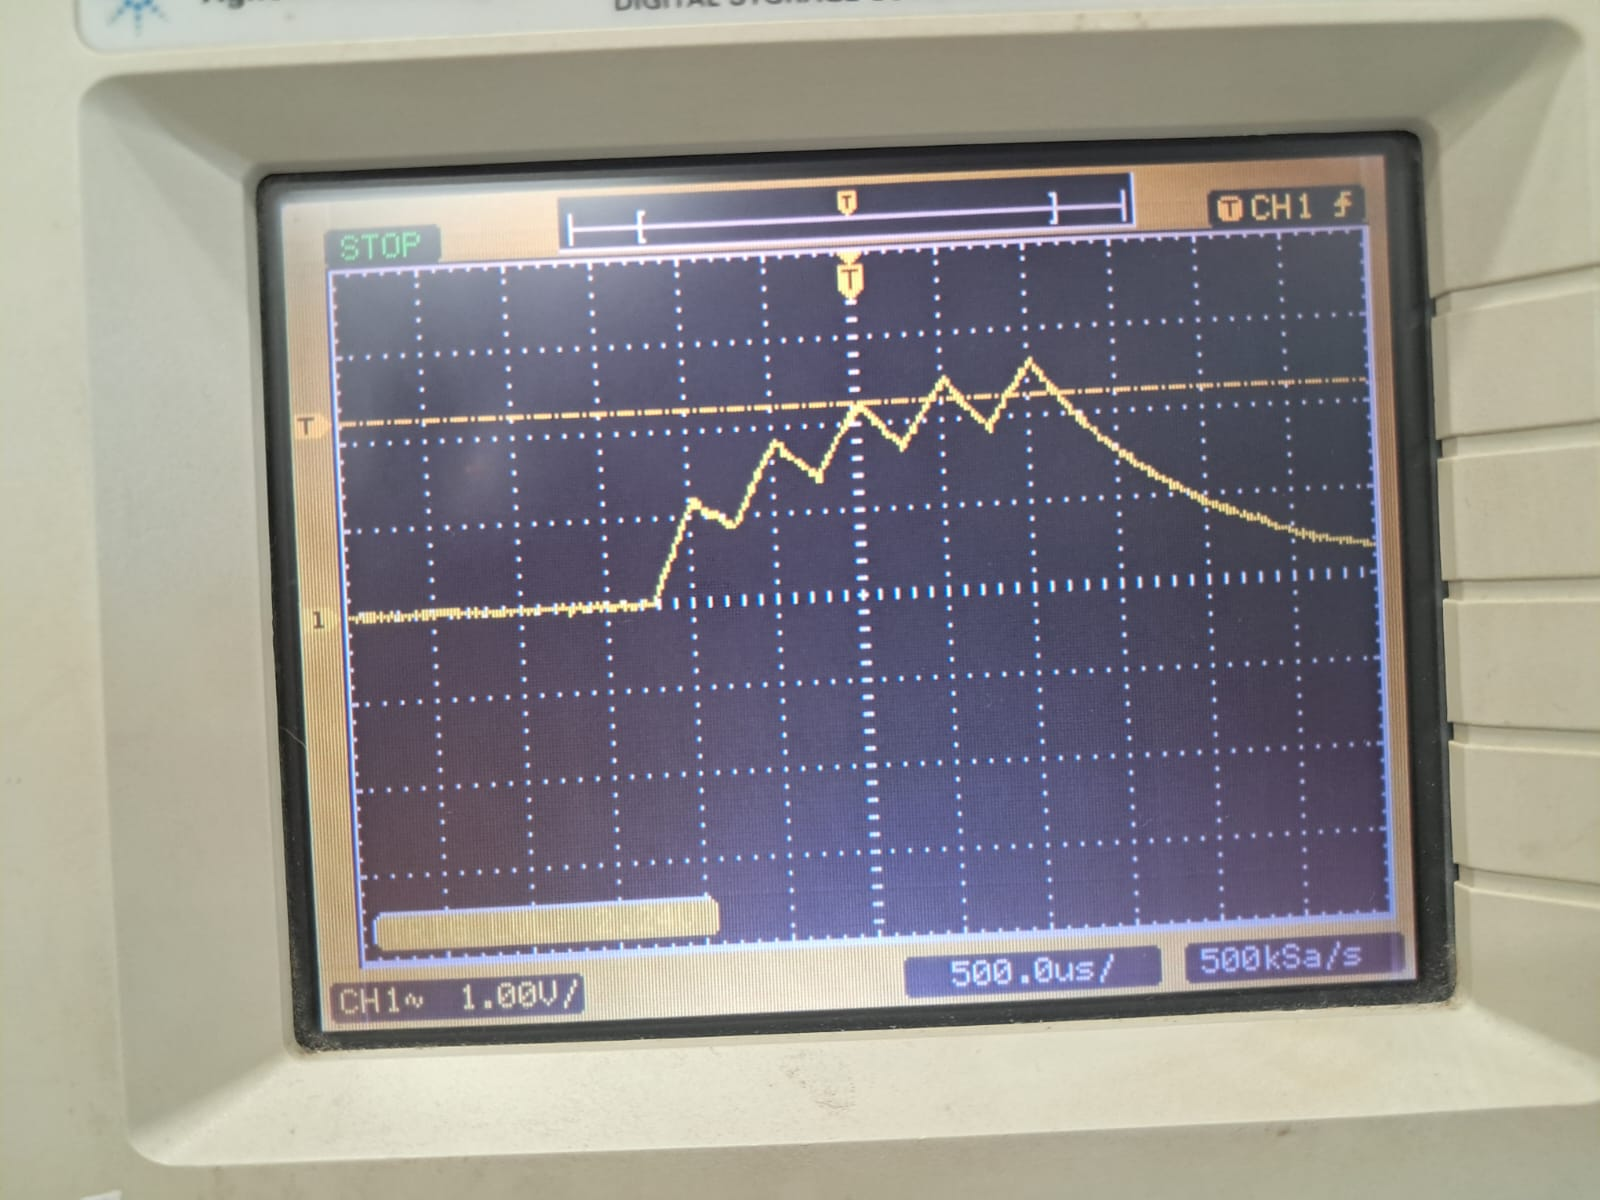
\includegraphics[width=\textwidth]{figs/T2kplot.jpeg}
    \end{minipage}
\end{figure}


\textbf{Explanation:}
The equation for charging of a capacitor is given by:
$$V_1=V_0(1-e^{-\frac{t}{\tau}})$$
$$V_1=5(1-e^{-\frac{10^{-4}}{2\times 10^{-3}}})$$
$$V_1=5(1-e^{-\frac{1}{20}})$$
$$V_1=1.776$$
Now the maximum value of the first peak is $1.776$V. 
Now, as the value of the signal from the function generator is zero, the capacitor starts discharging, with the peak value as $1.776$V.
The equation for discharging of a capacitor is:
$$V=V_0e^{-\frac{(t-(T/2))}{\tau}}$$
$$V_2=1.776 \times e^{-\frac{t-10^{-4}/2}{10^{-3}}}$$
$$V_2=1.776 \times e^{-\frac{10^{-4}-10^{-4}/2}{10^{-3}}}$$
$$V_2=1.3837$$
Now, we again send a signal of $5$V.
On solving the differential equation corresponding to a series RC circuit with initial conditions, we get:\\
$$v=V(1-e^{-\frac{t-t_0}{RC}})+v_0e^{-\frac{(t-t_0)}{RC}}$$
Here, $v_0=1.3837$\\
Hence, 
$V_3=5(1-\frac{1}{e^{\frac{1}{20}}})+1.3837(\frac{1}{e^{\frac{1}{20}}})$
$$V_3=2.1837$$
We notice that $V_3 > V_1$.
Again, now when the capacitor starts discharging, we get,
$$V_4=V_3e^{-\frac{t-(3T/2)}{\tau}}$$
$$V_4=1.7007$$
In the same way, we calculate the values of $V_5$, $V_6$ and so on.\\
As the number of cycles increases, the circuit is most likely going to reach steady state.

\begin{align}
    V_5&=2.4305\\
    V_6&=1.89\\
    V_7&=2.5801\\
    V_8&=2.0094\\
    V_9&=2.6709\\
    V_{10}&=2.0801\\
    v_{11}&=2.7260\\
\end{align}
We used lab.c code to iterate through these values. We notice that the steady state $V_{max}=2.810755$ and $V_{min}=2.189018$(after 38 iterations).
Given below is the steady state response of the circuit:
\begin{figure}[h]
    \centering
    \begin{minipage}{0.45\textwidth}
        \centering
        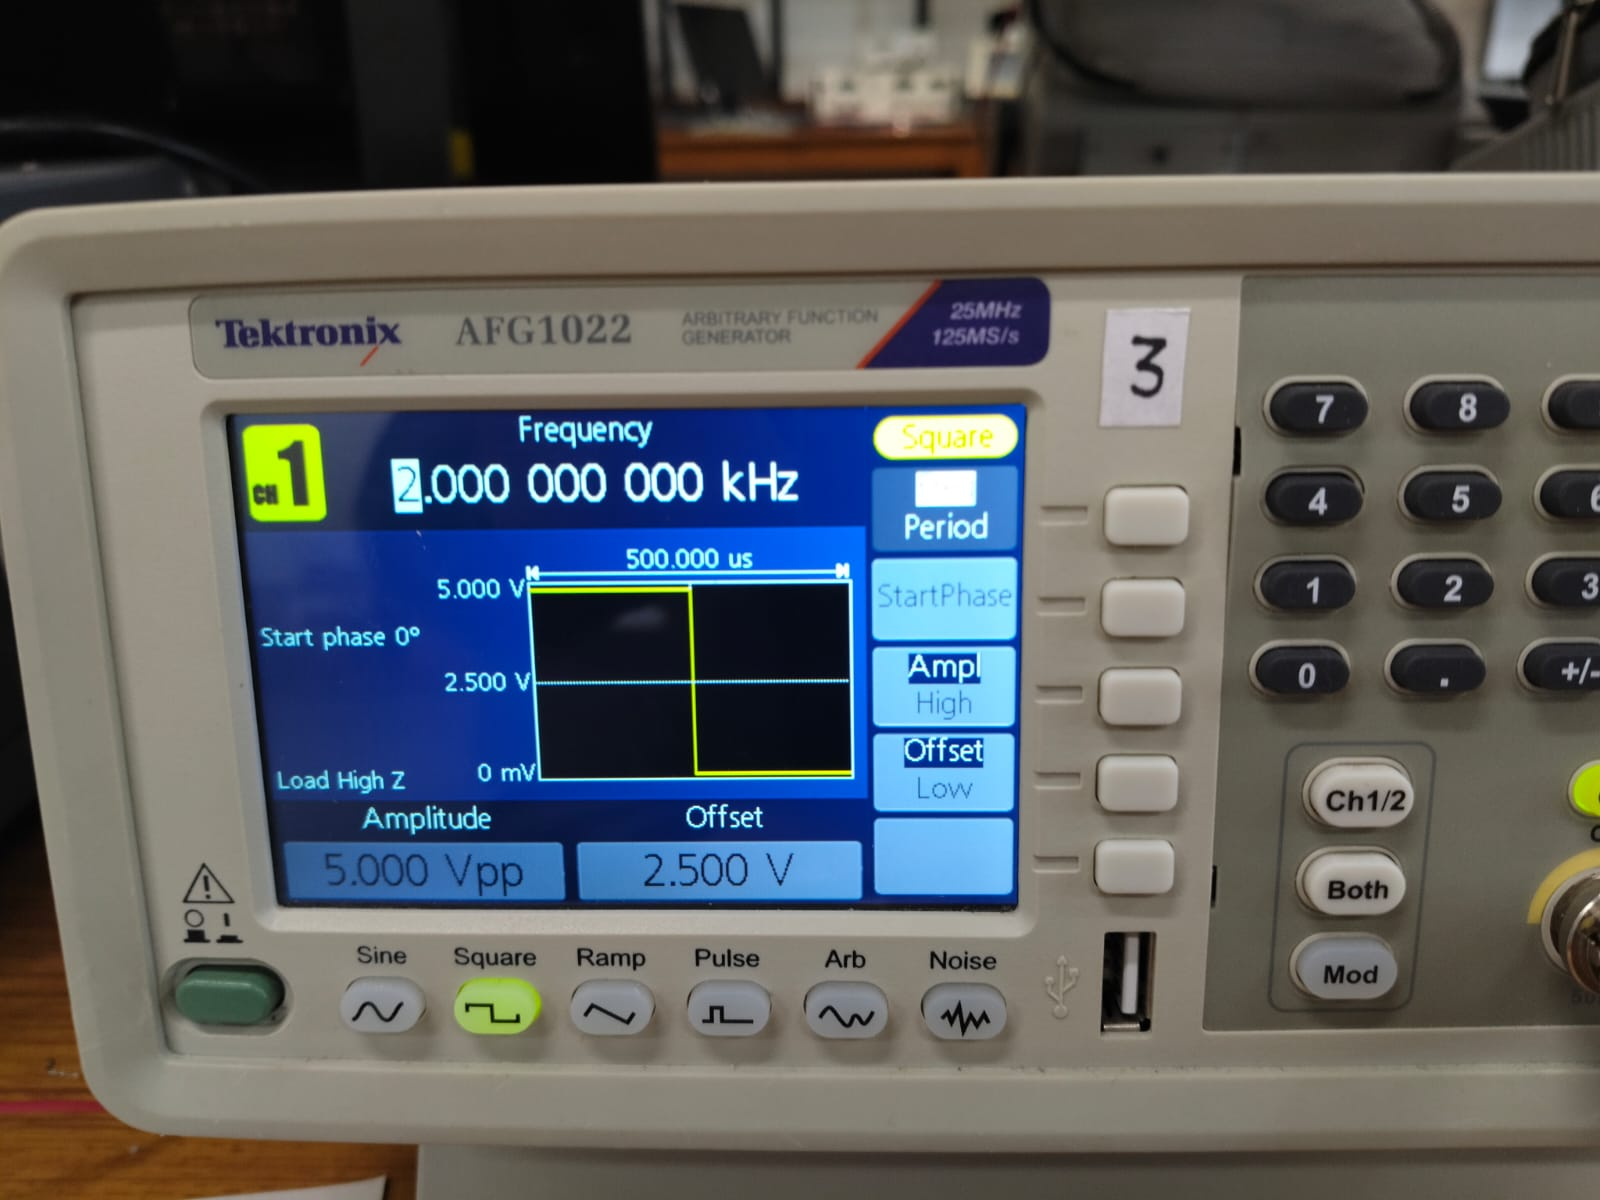
\includegraphics[width=\textwidth]{figs/C2kpara.jpeg}
    \end{minipage}\hfill
    \begin{minipage}{0.45\textwidth}
        \centering
        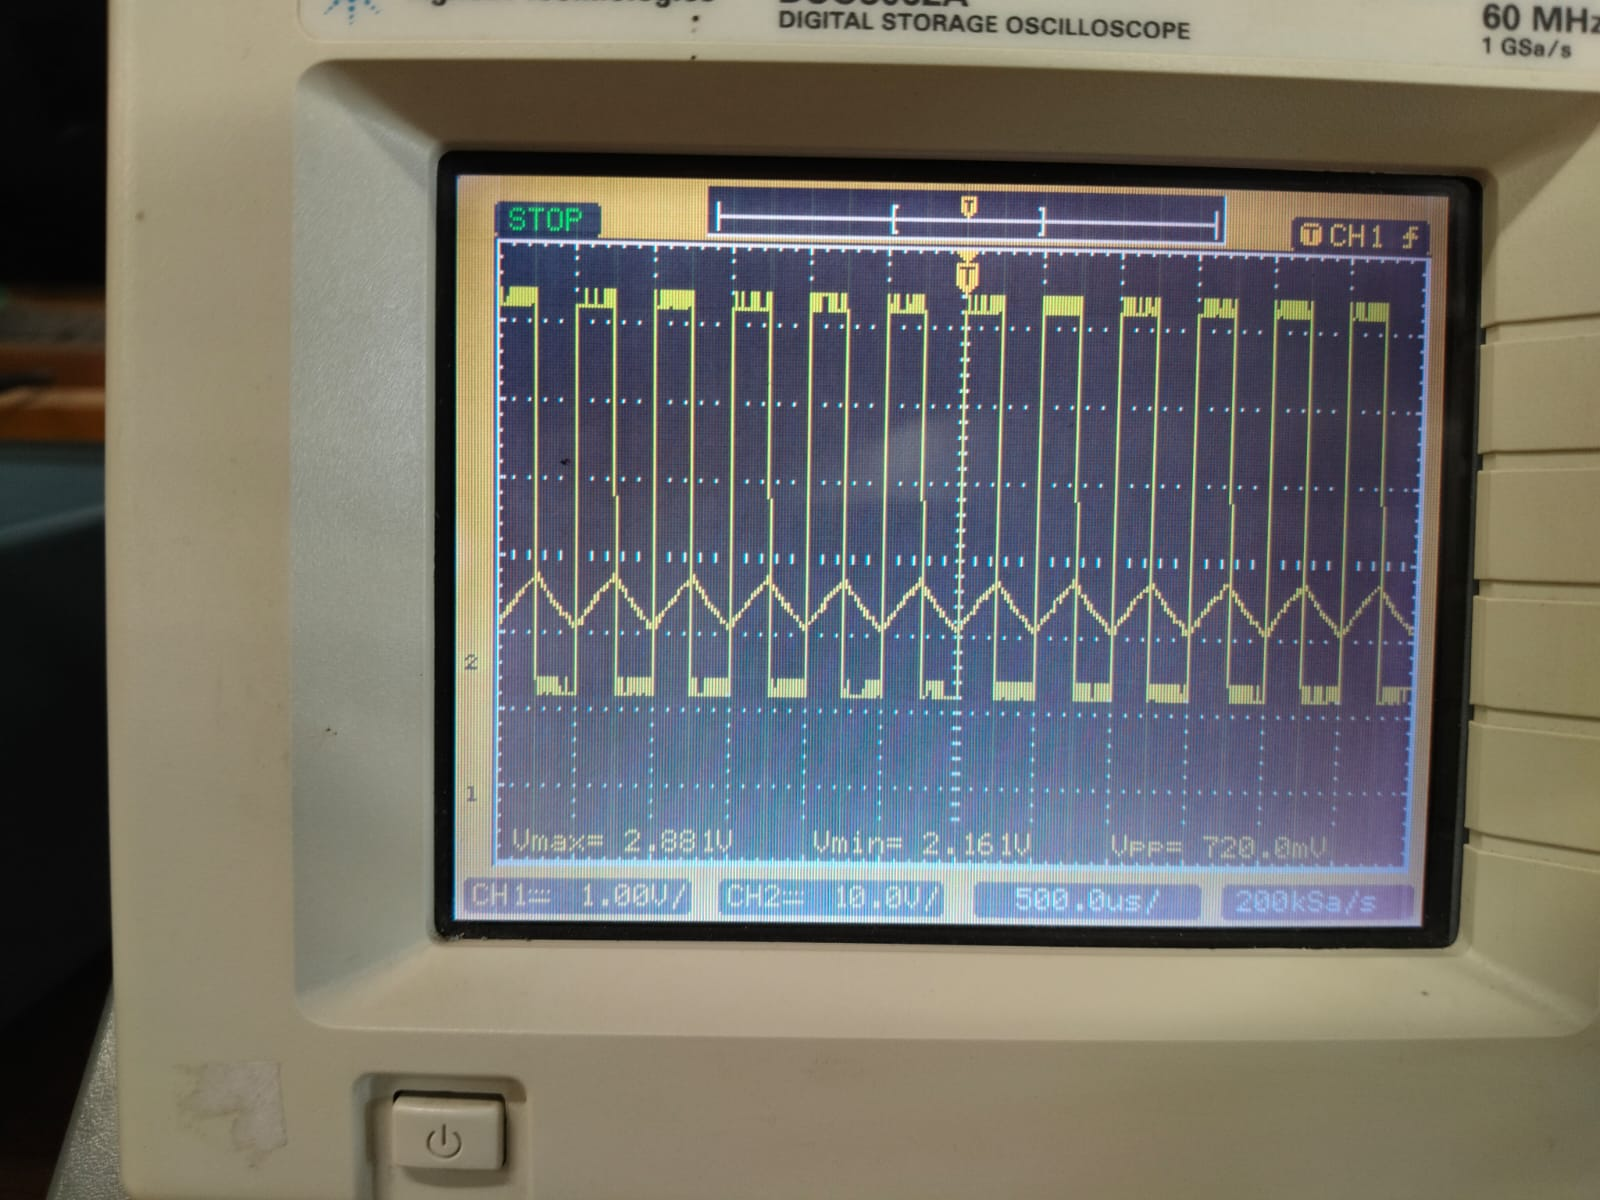
\includegraphics[width=\textwidth]{figs/C2kplot.jpeg}
    \end{minipage}
\end{figure}


\section{Conclusion}

In this experiment, we analyzed the response of an RC circuit to a square wave input by varying the time period relative to the circuit's time constant \( RC \). The observations demonstrate how the capacitor charges and discharges depending on the input signal frequency.

\begin{itemize}
    \item \textbf{For \( T >> RC \) (Low Frequency):}
    \begin{itemize}
        \item The capacitor has enough time to fully charge and discharge during each cycle.
        \item The circuit behaves almost like a DC system with minimal voltage drop across the capacitor after charging.
    \end{itemize}
    
    \item \textbf{For \( T = RC \) (Intermediate Frequency):}
    \begin{itemize}
        \item The capacitor does not fully charge or discharge within one cycle, resulting in a gradual buildup of voltage.
        \item The system reaches a steady-state oscillation with increasing peak voltages over multiple cycles.
    \end{itemize}
    
    \item \textbf{For \( T << RC \) (High Frequency):}
    \begin{itemize}
        \item The capacitor does not get enough time to charge significantly, causing small voltage fluctuations.
        \item The circuit behaves more like a resistive element, with minimal capacitive effects.
    \end{itemize}
\end{itemize}

These results align with the theoretical predictions for RC circuits and demonstrate the fundamental principles of transient and steady-state responses. Understanding such behavior is crucial in designing circuits for filtering, signal processing, and timing applications.


\end{document}

